\documentclass[12pt,a4paper]{article} 

\usepackage{fn2kursstyle}
\usepackage[russian]{babel}
\usepackage[T2A]{fontenc} 
\usepackage[utf8]{inputenc} 
\usepackage{geometry}
\usepackage{mathtools}
\usepackage{tikz}
\usepackage{chngcntr}

\counterwithout{equation}{section}
\counterwithout{figure}{section}
\graphicspath{{Pictures/}}
\frenchspacing 

\makeatletter
\newcommand*{\rom}[1]{\expandafter\@slowromancap\romannumeral #1@}
\makeatother

\title{Модель двух конкурирующих видов}
\group{ФН2-42Б}
\author{А.\,И.~Токарев}
\supervisor{М.\,П.~Галанин}
\date{2021}

\DeclareMathOperator{\Tr}{tr}

\newcommand*\circled[1]{\tikz[baseline=(char.base)]{
            \node[shape=circle,draw,inner sep=2pt] (char) {#1};}}

\makeatletter
\newenvironment{sqcases}{%
  \matrix@check\sqcases\env@sqcases
}{%
  \endarray\right.%
}
\def\env@sqcases{%
  \let\@ifnextchar\new@ifnextchar
  \left\lbrack
  \def\arraystretch{1.2}%
  \array{@{}l@{\quad}l@{}}%
}
\makeatother

\begin{document}
    \maketitle
    \tableofcontents
    \pagebreak

    \section-{Введение}
    В теории, если нет никаких факторов воздействия внешней среды на некоторую популяцию, то она способна размножаться вплоть до бесконечности. Однако в реальной жизни так не происходит, и особи разных видов так или иначе воздействуют друг на друга. И одним из таких типов взаимодействий является конкуренция. Ее разделяют на внутривидовую конкуренцию (соперничество между особями одного вида за жизненные ресурсы) и на межвидовую конкуренцию (взаимоотношение между популяциями двух (или более) видов, которое неблагоприятно сказывается на их росте и выживании). 

    Проблема динамики популяции заинтересовала ученых еще в \rom{18} веке. Именно тогда они начали заниматься разработкой методов, способных описать динамику роста и сокращения популяций живых организмов.
    
    Основателем современной математической теории популяций справедливо считается Вито Вольтерра\footnote{В.\,Вольтерра (\textit{ит.} Vito Volterra, 1860--1940) --- итальянский математик и физик.}, разработавший математическую теорию биологических сообществ, аппаратом которой служат дифференциальные и интегро-дифференциальные уравнения. Эта модель основывается на следующих гипотезах:
    \begin{enumerate}
        \item Пища имеется в неограниченном количестве или ее поступление регулируется.
        \item В единицу времени погибает одинаковое количество особей одного вида.
        \item Прирост численности вида пропорционален его текущей численности.
    \end{enumerate}

    \section{Постановка задачи}
    Рассмотрим задачу из области динамики популяций. Пусть есть два сходных вида, конкурирующих между собой за пищу. Очевидно, что возможны следующие варианты: 
    \pagebreak
    \begin{itemize}
        \item Выживает только первый вид.
        \item Выживает только второй вид.
        \item Выживают оба вида.
        \item Оба вида вымирают.
    \end{itemize}
    
    Каждый из этих вариантов соответствует наличию своего положения равновесия. Тем самым для описания данной системы нужна модель с четырьмя стационарными точками --- стационарными состояниями системы.

    В соответствии с гипотезами В.\,Вольтерра модель двух конкурирующих видов выглядит следующим образом:
    \begin{equation}
        \label{volterra}
        \begin{cases}
            \dfrac{dx_1}{dt} = a_1 x_1 - b_{12} x_1 x_2 - c_1 {x_1}\!^2,
            \\[1em]
            \dfrac{dx_2}{dt} = a_2 x_2 - b_{21} x_2 x_1 - c_2 {x_2}\!^2 ,
        \end{cases}
    \end{equation}
    \noindent где $a_1, a_2$ --- коэфициенты скорости роста популяции; $b_{12}, b_{21}$ --- коэфициенты межвидовой борьбы; $c_1, c_2$ --- внутривидовой борьбы первого и второго вида соответственно.

    В данной курсовой работе необходимо рассмотреть все варианты параметров системы и исследовать качественное поведение ее решений. Также важно уделить внимание особым точкам системы.

    \section{Стационарные состояния}

    Найдем стационарные точки. Для этого необходимо решить систему уравнений вида: 
    \begin{equation}
        \label{seps}
        \begin{cases}
            a_1 x_1 - b_{12} x_1 x_2 - c_1 {x_1}\!^2 = x_1 (a_1 - b_{12} x_2 - c_1 x_1) = 0,
            \\
            a_2 x_2 - b_{21} x_2 x_1 - c_2 {x_2}\!^2 = x_2 (a_2 - b_{21} x_1 - c_2 x_2) = 0,
        \end{cases}
    \end{equation}
    
    \noindent откуда получаем 4 стационарных состояния:
    \begin{enumerate}
        \setlength\itemsep{0.5em}
        \item $ x_1 = 0,\ x_2 = 0 $ --- вымирание обоих видов.
        \item $ x_1 = 0,\ x_2 = \dfrac{a_2}{c_2} $ --- вымирание первого вида, достижение вторым видом конечной численности $ \dfrac{a_2}{c_2} $.
        \item $ x_1 = \dfrac{a_1}{c_1},\ x_2 = 0 $ --- противоположная ситуация, то есть достижение первым видом численности $ \dfrac{a_1}{c_1} $ и вымирание второго вида.
        \item $ x_1 = \dfrac{a_1 c_2 - a_2 b_{12}}{c_1 c_2 - b_{12} b_{21}},\ x_2 = \dfrac{a_2 c_1 - a_1 b_{21}}{c_1 c_2 - b_{12} b_{21}}$ --- выживание обоих видов.
    \end{enumerate} 

    \vspace{1em}Особое внимание стоит уделить последнему стационарному состоянию. Решения $ x_1,\ x_2 $ в этой ситуации должны быть положительными, в противном случае система теряет биологический смысл, потому что число особей в популяции не может быть отрицательным. Условие положительности выполняется в одной из двух ситуаций: 
    \begin{equation}
        \label{positive}
        \begin{cases}
            a_1 c_2 > a_2 b_{12},
            \\
            a_2 c_1 > a_1 b_{21},
            \\
            c_1 c_2 > b_{12} b_{21},
        \end{cases}
    \end{equation}
    \noindent или
    \begin{equation}
        \label{negative}
        \begin{cases}
            a_1 c_2 < a_2 b_{12},
            \\
            a_2 c_1 < a_1 b_{21},
            \\
            c_1 c_2 < b_{12} b_{21},
        \end{cases}
    \end{equation}

    \noindent при этом третье неравенство следует из первого и второго в обоих случаях.

    Возникновение тех или иных стационарных состояний, упомянутых выше, зависит от исходных параметров системы (\refeq{volterra}). Для того, чтобы получить более наглядное представление о всех возможных ситуацях, которые могут возникнуть в зависимости от этих параметров, можно построить график \linebreak прямых-сепаратрис. Их можно вывести из системы (\refeq{seps}):
    \begin{equation}
        \label{nullclines}
            x_1 = 0,\qquad 
            x_2 = 0,\qquad
            x_2 = \dfrac{a_2 + b_{21} x_1}{c_2},\qquad 
            x_2 = \dfrac{a_1 + c_1 x_1}{b_{12}}.
    \end{equation}
    Попарные пересечения сепаратрис дают стационарные состояния. Возможные взаимные расположения прямых-сепаратрис продемонстрированы на рис. \refeq{fig:sep_1}-\refeq{fig:sep_2}:
  
    \begin{figure}
        \centering
        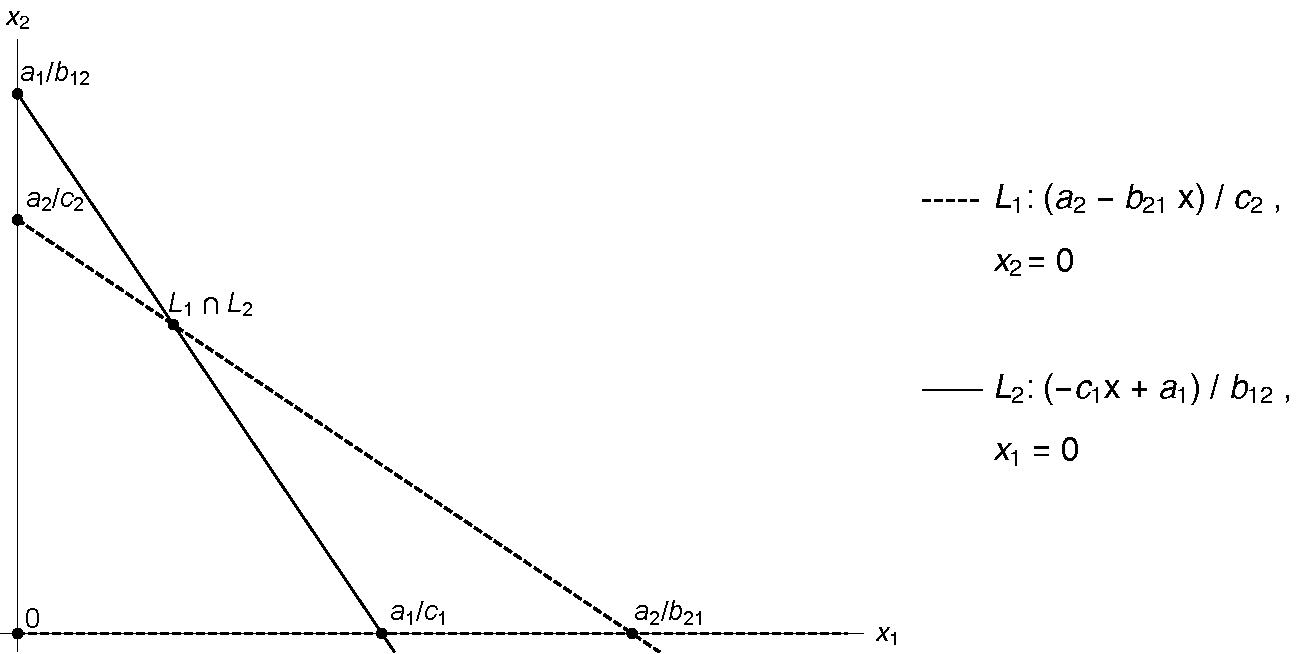
\includegraphics[width=\textwidth]{sep_1.pdf}
        \caption{Расположение прямых-сепаратрис, когда числитель и знаменатель положительные}
        \label{fig:sep_1}
    \end{figure}

    \begin{figure}
        \centering
        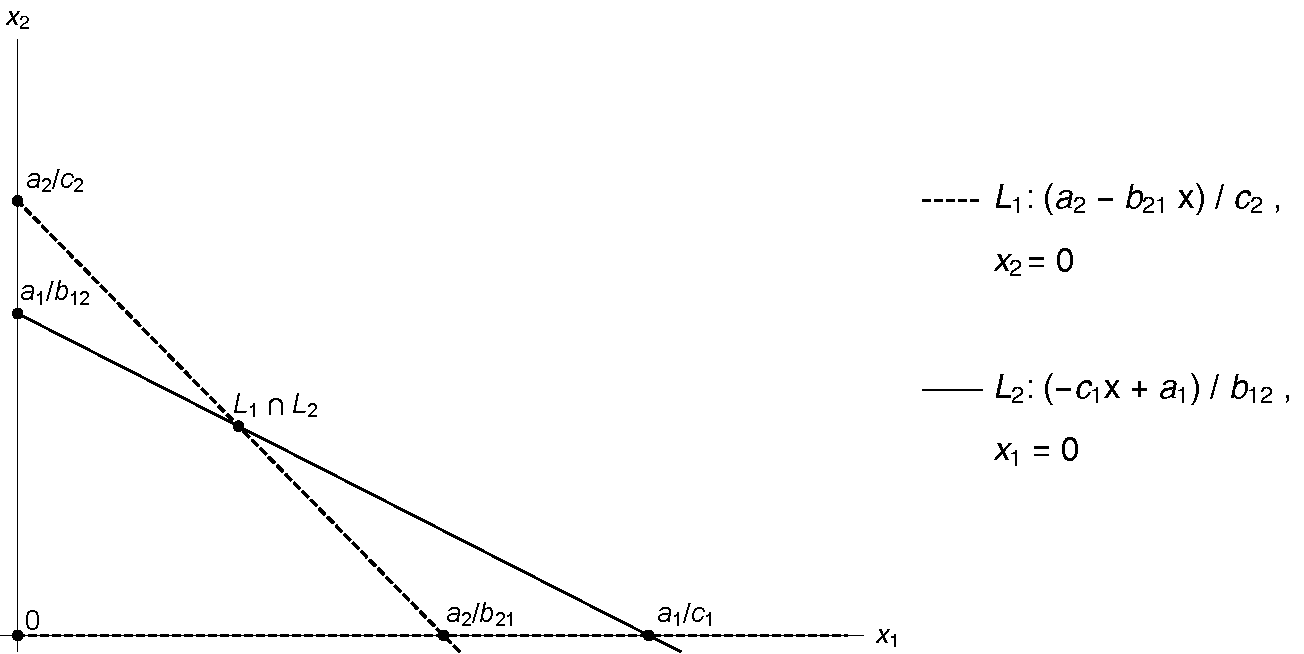
\includegraphics[width=\textwidth]{sep_2.pdf}
        \caption{Расположение прямых-сепаратрис, когда числитель и знаменатель отрицательные}
        \label{fig:sep_2}
    \end{figure}

    \pagebreak

    \section{Линеаризация системы в окрестности стационарных точкек}
    В общем виде линеаризованную систему можно представить в виде матрицы Якоби следющего вида: 
    \begin{equation}
        \label{jacobian}
        \mathbb{J} = 
            \begin{pmatrix}
                \dfrac{\partial{\dot x_1}}{\partial x_1}
                &
                \dfrac{\partial{\dot x_1}}{\partial x_2}
                \\[5mm]
                \dfrac{\partial{\dot x_2}}{\partial x_1}
                &
                \dfrac{\partial{\dot x_2}}{\partial x_2}
            \end{pmatrix}
        =
            \begin{pmatrix}
                a_1 - b_{12} x_2 - 2 c_1 x_1 & -b_{12} x_1
                \\
                -b_{21} x_2 & a_2 - b_{21} x_1 - 2c_2 x_2
            \end{pmatrix}\!.
    \end{equation}

    Линеаризуем систему в окрестности всех четырех стационарных точек:
    \[
        \mathbb{J}_{\rom 1} = 
                \begin{pmatrix}
                    a_1 & 0
                    \\
                    0   & a_2
                \end{pmatrix}\!,\quad
        \mathbb{J}_{\rom 2} = 
            \begin{pmatrix}
                -a_1 & -\dfrac{a_1 b_{12}}{c_1}
                \\[4mm]
                0   & \dfrac{a_2 c_1 - a_1 b_{21}}{c_1}
            \end{pmatrix}\!,\quad
        \mathbb{J}_{\rom 3} = 
            \begin{pmatrix}
                \dfrac{a_1 c_2 - b_{12} a_2}{c_2} & 0
                \\[4mm]
                -\dfrac{a_2 b_{21}}{c_2}          & -a_2
            \end{pmatrix}\!,
    \]

    \[
        \mathbb{J}_{\rom 4} = 
            \begin{pmatrix}
            \dfrac{c_1 (a_1 c_2 - a_2 b_{12})}{b_{12} b_{21} - c_1 c_2} & \dfrac{b_{12} (a_1 c_2 - a_2 b_{12})}{b_{12} b_{21} - c_1 c_2}
                \\[4mm]
                \dfrac{b_{21} (a_2 c_1 - a_1 b_{21})}{b_{12} b_{21} - c_1 c_2}   & \dfrac{c_2 (a_2 c_1 - a_1 b_{21})}{b_{12} b_{21} - c_1 c_2}
            \end{pmatrix}\!,
    \]
    \\
    и вспомним, что в зависимости от исходных параметров системы выполняется одно из двух условий(\refeq{positive}, \refeq{negative}), определящих типы этих точек. 

    \section{Фазовые портреты}
    Все стационарные точки являются простыми, поэтому их тип определяется собственными числами матриц $ \mathbb{J}_{\rom 1 - \rom 4}.$

    \subsection{Первый вариант параметров системы.}

    С учетом условий \eqref{positive}:

    \begin{enumerate}
        \setlength\itemsep{0.5em}
        \item $ \lambda_1 = a_1 > 0,\ \lambda_2 = a_2 > 0 \Rightarrow $ точка $ (0, 0) $ --- неустойчивый узел.
    
        \item $ \lambda_1 = -a_1 < 0,\ \lambda_2 = \dfrac{a_2 c_1 - a_1 b_{21}}{c_1} > 0 \Rightarrow $ точка $ \left( \dfrac{a_1}{c_1}, 0 \right) $ --- седло.
        
        \item  $ \lambda_1 = \dfrac{a_1 c_2 - b_{12} a_2}{c_2} > 0,\ \lambda_2 = -a_2 < 0 \Rightarrow $ точка $ \left( 0, \dfrac{a_2}{c_2} \right) $ --- седло.
        
        \item Для того, чтобы определить тип последней стационарной точки, следует решить квадратное уравнение вида:
        \[
            \begin{vmatrix}
                a_{11} - \lambda & a_{12}
                \\
                a_{21} & a_{22} - \lambda
            \end{vmatrix} = 
                \lambda^2 - \lambda(a_{11} + a_{22}) + (a_{11} a_{22} - a_{12} a_{21}) = 0,
        \]

        \noindent где $ a_{ij} $ --- коэфициенты матрицы $ \mathbb{J}_{\rom 4} $,  $ (a_{11} + a_{22}) = \Tr { \mathbb{J}_{\rom 4} } $ --- след этой матрицы,   $ (a_{11} a_{22} - a_{12} a_{21}) = \det \mathbb{J}_{\rom 4} $ --- ее определитеть. Проанализируем знаки собственных чисел $ \lambda_1 $ и $ \lambda_2 $, воспользовавшись теоремой Виета:
        \[
          \begin{cases}
            \lambda_1 + \lambda_2 = a_{11} + a_{22} = \dfrac{c_1 (a_1 c_2 - b_{12} a_2) + c_2 (a_2 c_1 - a_1 b_{21})}{b_{12} b_{21} - c_1 c_2} & (\Delta),
            \\[1.5em]
            \lambda_1 \cdot \lambda_2 = a_{11} a_{22} - a_{12} a_{21} = \dfrac{(a_1 c_2 - b_{12} a_2)(a_2 c_1 - b_{21} a_1)}{c_1 c_2 - b_{12} b_{21}} & (\Delta \Delta)
          \end{cases}  
        \]
 
        \[
            \begin{split}
                (\Delta) & \colon \lambda_1 + \lambda_2 = a_{11} + a_{22} = \dfrac{c_1 (a_1 c_2 - b_{12} a_2) + c_2 (a_2 c_1 - a_1 b_{21})}{b_{12} b_{21} - c_1 c_2} < 0, 
                \\
                (\Delta \Delta) & \colon \lambda_1 \cdot \lambda_2 > 0 \Rightarrow \text {собственные числа имеют одинаковый знак},
            \end{split}
        \]
        \noindent а так как $ \lambda_1 + \lambda_2 $ < 0 и $ \lambda_1,\, \lambda_2 $ имеют один и тот же знак, то они оба отри-\\[0.4em]цательные. Значит,  точка $ \left( \dfrac{a_1 c_2 - a_2 b_{12}}{c_1 c_2 - b_{12} b_{21}}, \dfrac{a_2 c_1 - a_1 b_{21}}{c_1 c_2 - b_{12} b_{21}} \right) $ --- устойчивый узел.
    \end{enumerate}

    Имеем только одно устойчивое состояние. Осталось построить фазовый портрет. Для этого сначала построим поля направлений для $ \dot x_1 $ и $ \dot x_2 $, чтобы определить знаки этих проивзодных в каждой из подобластей рис. \refeq{fig:sep_1}.

    Общее поле направлений (рис. \refeq{fig:areas_1}) получается путем объединения полей направлений для $ \dot x_1 $ (рис. \refeq{fig:dirFields_11}) и $ \dot x_2 $ (рис. \refeq{fig:dirFields_12}):

    \begin{itemize}
        \setlength\itemsep{0.4em}
        \item В первой области $ \dot x_1 > 0 $ и $ \dot x_2 > 0 \, \Rightarrow $ общие траектории направлены вправо вверх;
        \item Во второй области $ \dot x_1 > 0 $ и $ \dot x_2 < 0 \, \Rightarrow $ общие траектории направлены вправо вниз;
        \item В третьей области $ \dot x_1 < 0 $ и $ \dot x_2 < 0 \, \Rightarrow $ общие траектории направлены влево вниз;
        \item В четвертой области $ \dot x_1 < 0 $ и $ \dot x_2 > 0 \, \Rightarrow $ общие траектории направлены влево вверх.
    \end{itemize}

    \begin{figure}[h]
        \centering
        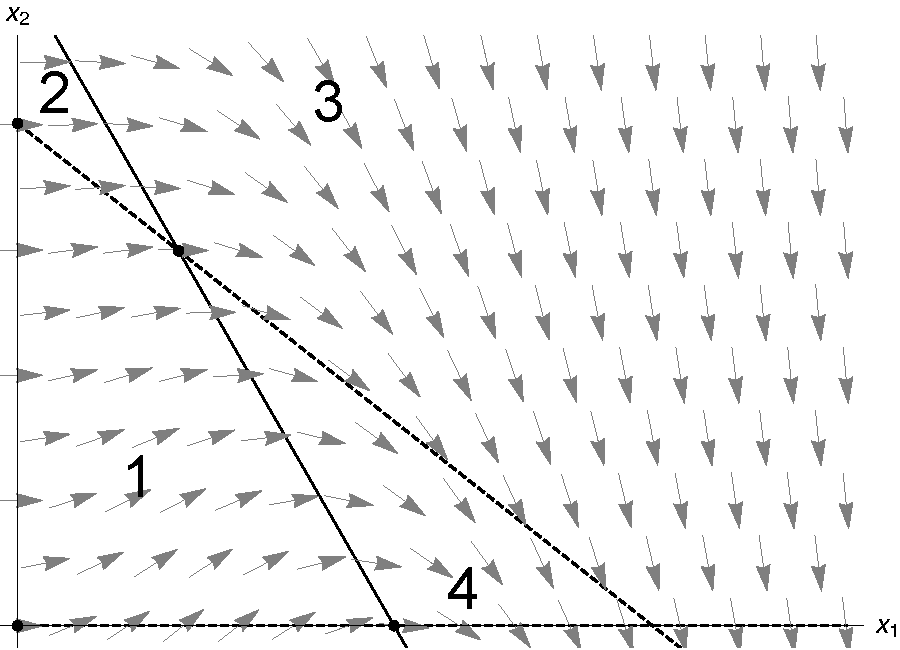
\includegraphics[width=0.64\textwidth]{dirFields_11.pdf}
        \caption{Поле направлений для $ \dot x_1 $}
        \label{fig:dirFields_11}
    \end{figure}

    \begin{figure}[h]
        \centering
        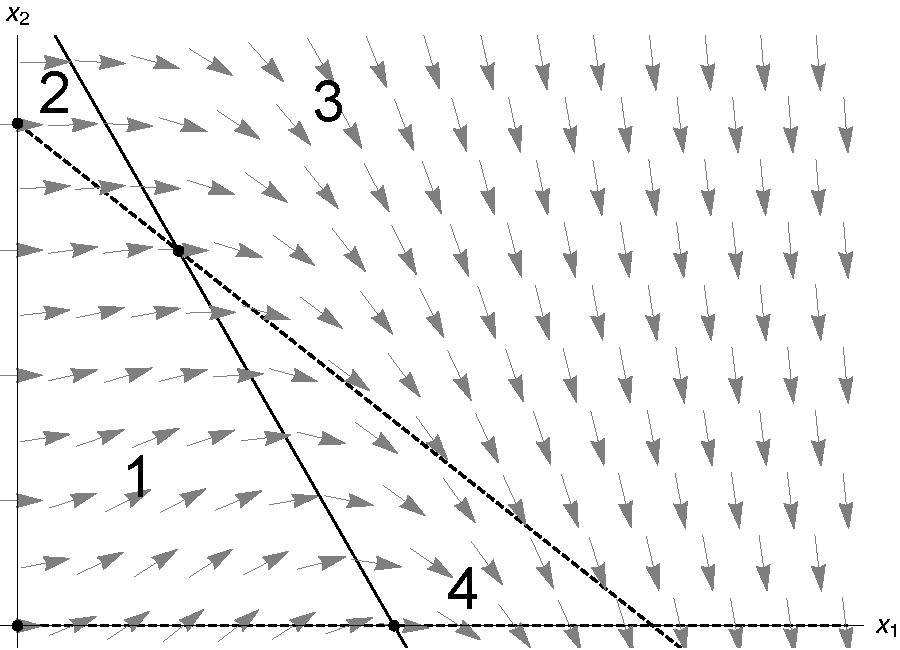
\includegraphics[width=0.64\textwidth]{dirFields_12.pdf}
        \caption{Поле направлений для $ \dot x_2 $}
        \label{fig:dirFields_12}
    \end{figure}

    \pagebreak
    
    \begin{figure}[h]
        \centering
        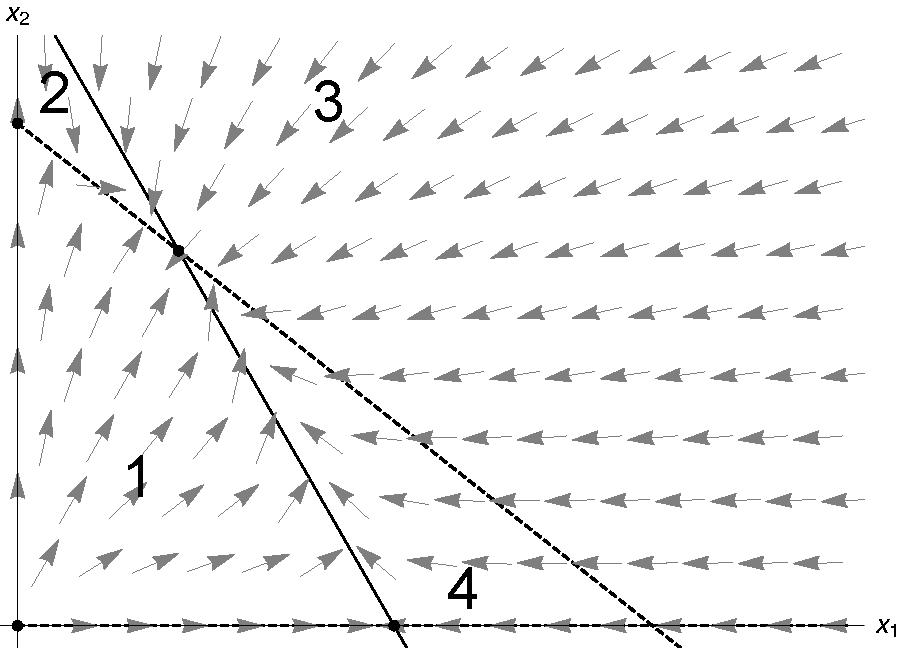
\includegraphics[width=0.64\textwidth]{areas_1.pdf}
        \caption{Общие направления траекторий}
        \label{fig:areas_1}
    \end{figure}

    \begin{figure}[h]
        \centering
        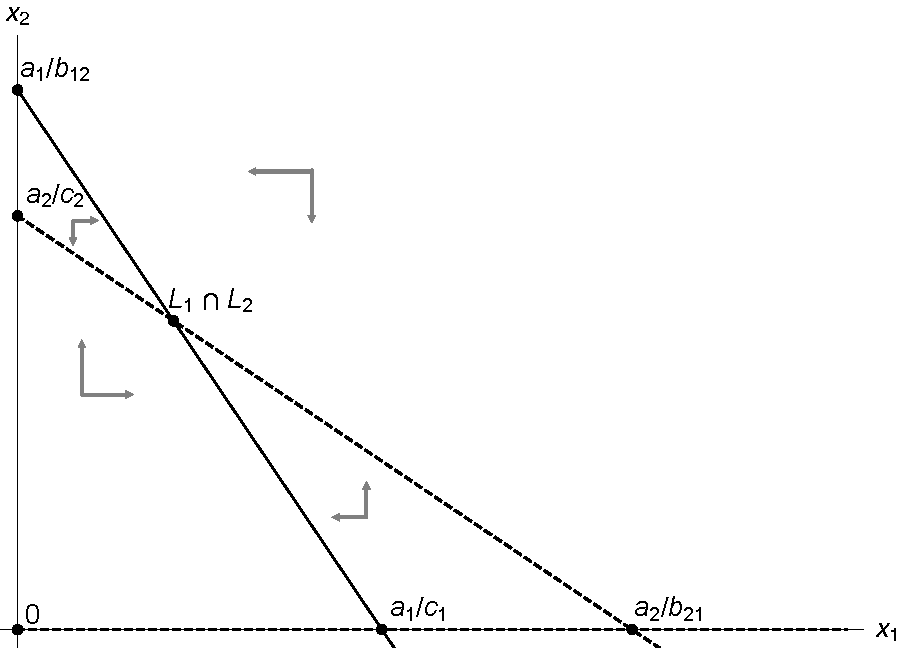
\includegraphics[width=0.64\textwidth]{areas_1*.pdf}
        \caption{Картина направлений движения траекторий}
        \label{fig:areas_1*}
    \end{figure}

    \pagebreak

    Воспользуемся системой компьютерной алгебры Wolfram Mathematica для того, чтобы построить окончательный фазовый портрет:
    \begin{figure}[h]
        \centering
        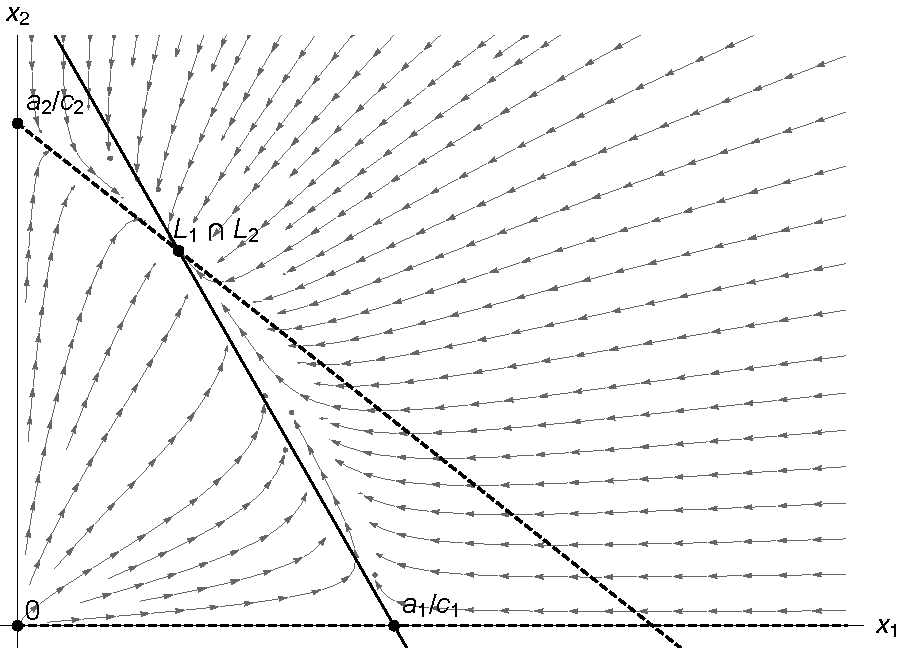
\includegraphics[width=0.7\textwidth]{phase_1.pdf}
        \caption{Сосуществование двух видов}
        \label{fig:phase_1}
    \end{figure}

    Из полученной картины можно сделать вывод, что сосуществование двух видов  гарантировано, потому что все траектории стремятся к 4-ой точке.

    \subsection{Второй вариант параметров системы}

    С учетом условий \eqref{negative}: 

    \begin{enumerate}
        \setlength\itemsep{0.5em}
        \item $ \lambda_1 = a_1 > 0,\ \lambda_2 = a_2 > 0 \Rightarrow $ точка $ (0, 0) $ --- неустойчивый узел.
    
        \item $ \lambda_1 = -a_1 < 0,\ \lambda_2 = \dfrac{a_2 c_1 - a_1 b_{21}}{c_1} < 0 \Rightarrow $ точка $ \left( \dfrac{a_1}{c_1}, 0 \right) $ --- устойчивый узел.
        
        \item  $ \lambda_1 = \dfrac{a_1 c_2 - b_{12} a_2}{c_2} < 0,\ \lambda_2 = -a_2 < 0 \Rightarrow $ точка $ \left( 0, \dfrac{a_2}{c_2} \right) $ --- устойчивый узел.
        
        \item $ \det \mathbb{J}_{\rom 4}\! < \!0 \Rightarrow$ собственные значения имеют разные знаки, а значит точка-пересечение сепаратрис $ \left( \dfrac{a_1 c_2 - a_2 b_{12}}{c_1 c_2 - b_{12} b_{21}}, \dfrac{a_2 c_1 - a_1 b_{21}}{c_1 c_2 - b_{12} b_{21}} \right) $ --- седло.
        \\
    \end{enumerate}

    Получили два устойчивых узла и один неустойчивый, которые разделены седлом. Как и в предыдущем случае, продемонстрируем направления траекторий в каждой из подобластей:

    \begin{itemize}
        \setlength\itemsep{0.4em}
        \item В первой области $ \dot x_1 > 0 $ и $ \dot x_2 > 0 \, \Rightarrow $ траектории направлены вправо вверх;
        \item Во второй области $ \dot x_1 < 0 $ и $ \dot x_2 > 0 \, \Rightarrow $ траектории направлены влево вверх;
        \item В третьей области $ \dot x_1 < 0 $ и $ \dot x_2 < 0 \, \Rightarrow $ траектории направлены влево вниз;
        \item В четвертой области $ \dot x_1 > 0 $ и $ \dot x_2 < 0 \, \Rightarrow $ траектории направлены вправо вниз.
    \end{itemize}

    \begin{figure}[h]
        \centering
        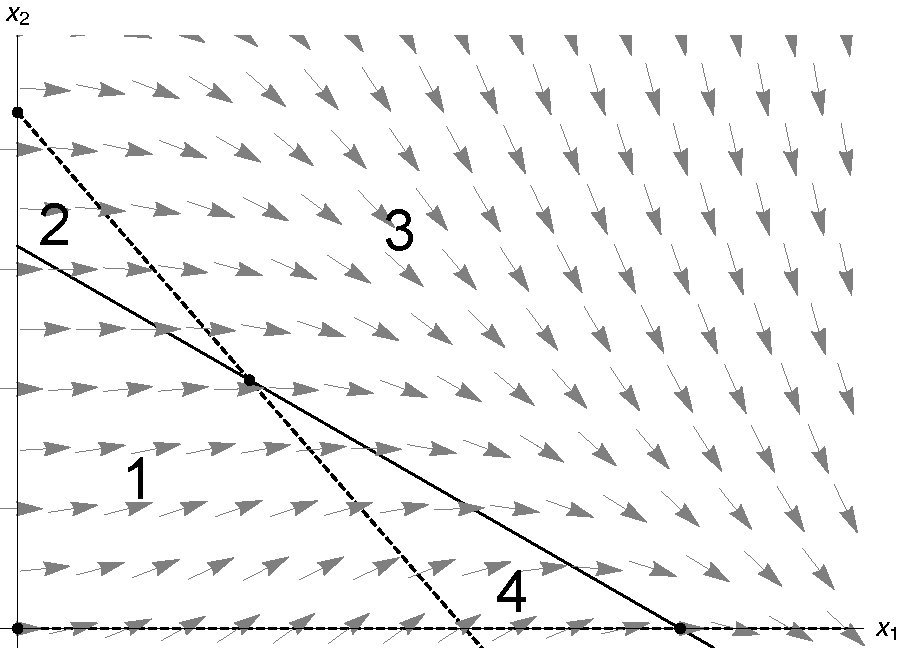
\includegraphics[width=0.64\textwidth]{dirFields_21.pdf}
        \caption{Поле направлений для $ \dot x_1 $}
        \label{fig:dirFields_21}
    \end{figure}

    \pagebreak

    \begin{figure}[h]
        \centering
        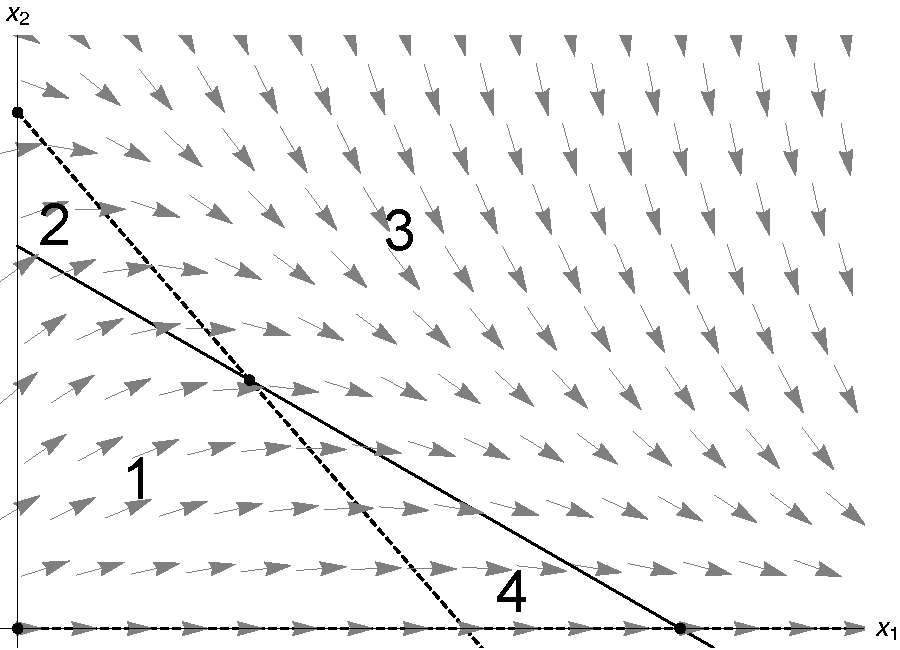
\includegraphics[width=0.64\textwidth]{dirFields_22.pdf}
        \caption{Поле направлений для $ \dot x_2 $}
        \label{fig:dirFields_22}
    \end{figure}
    
    \begin{figure}[h]
        \centering
        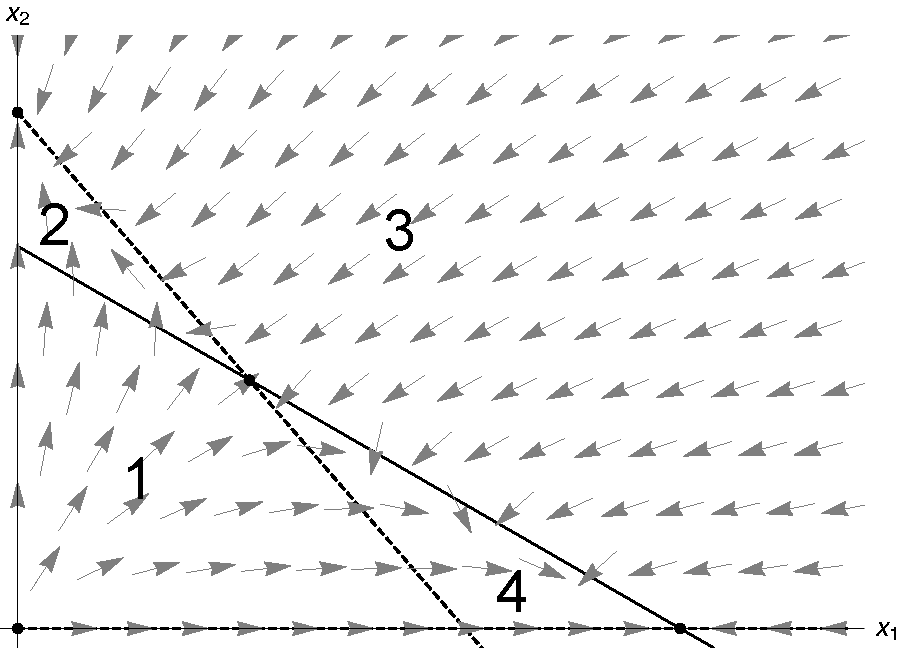
\includegraphics[width=0.64\textwidth]{areas_2.pdf}
        \caption{Общие направления траекторий}
        \label{fig:areas_2}
    \end{figure}

    \pagebreak

    \begin{figure}[h]
        \centering
        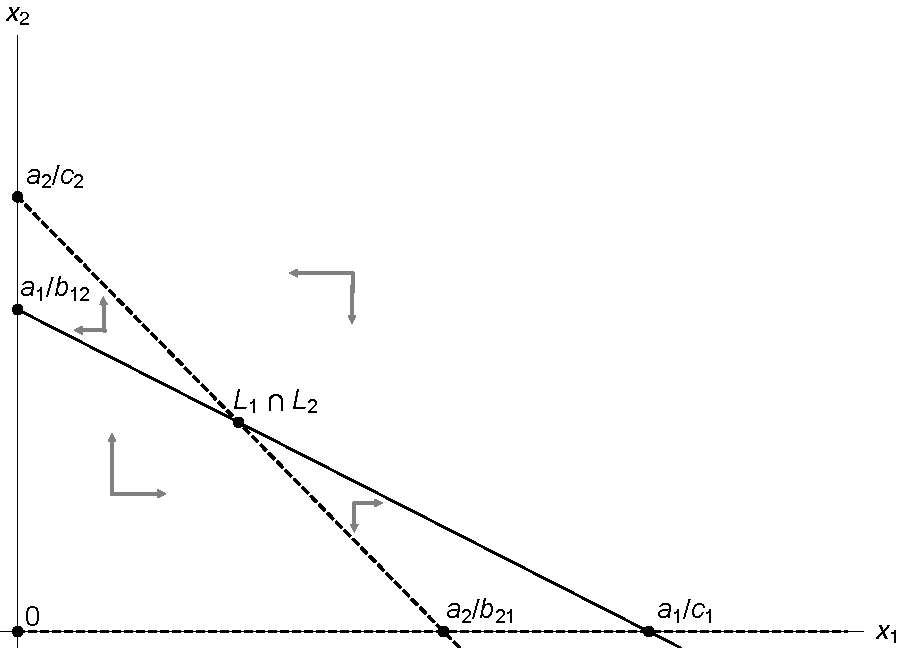
\includegraphics[width=0.64\textwidth]{areas_2*.pdf}
        \caption{Картина направлений движения траекторий}
        \label{fig:areas_2*}
    \end{figure}
    
    Значит, фазовый потрет выглядит следующим образом:
    \begin{figure}[h]
        \centering
        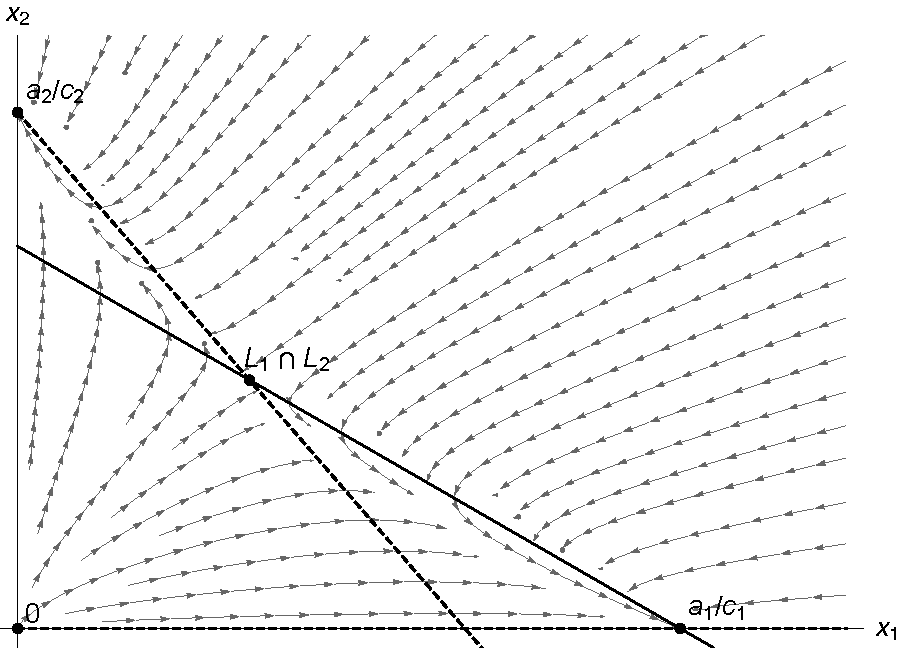
\includegraphics[width=0.64\textwidth]{phase_2.pdf}
        \caption{Выживание одного из двух конкурирующих видов}
        \label{fig:phase_2}
    \end{figure}

    Таким образом, сосуществование двух конкурирующих видов крайне маловероятно. Большинство траекторий стремятся либо ко 2-ой, либо к 3-ей точке. А они соответствуют выживанию лишь одного из видов.

    \section{Дополнительные случаи}
    Опишем ситуации, когда не выполняется ни одно из условий (\ref{positive},\,\ref{negative}), то есть когда точка пересечения сепаратрис находится вне $1^{\text{го}}$ квадранта (или ее вовсе нет, если прямые параллельные). Тогда эту точку можно исключить из рассмотрения, потому что число особей не может быть отрицательным. Значит, будем рассматривать один из двух случаев:
    \begin{equation}
        \label{posneg}
        \begin{cases}
            a_1 c_2 > a_2 b_{12},
            \\
            a_2 c_1 < a_1 b_{21},
        \end{cases}
    \end{equation}
    \noindent или
    \begin{equation}
        \label{negpos}
        \begin{cases}
            a_1 c_2 < a_2 b_{12},
            \\
            a_2 c_1 > a_1 b_{21}
        \end{cases}
    \end{equation}

    \subsection{Первый случай}
    При выполнении условий \eqref{posneg} график прямых-сепаратрис выглядит следующим образом:
    \begin{figure}[h]
        \centering
        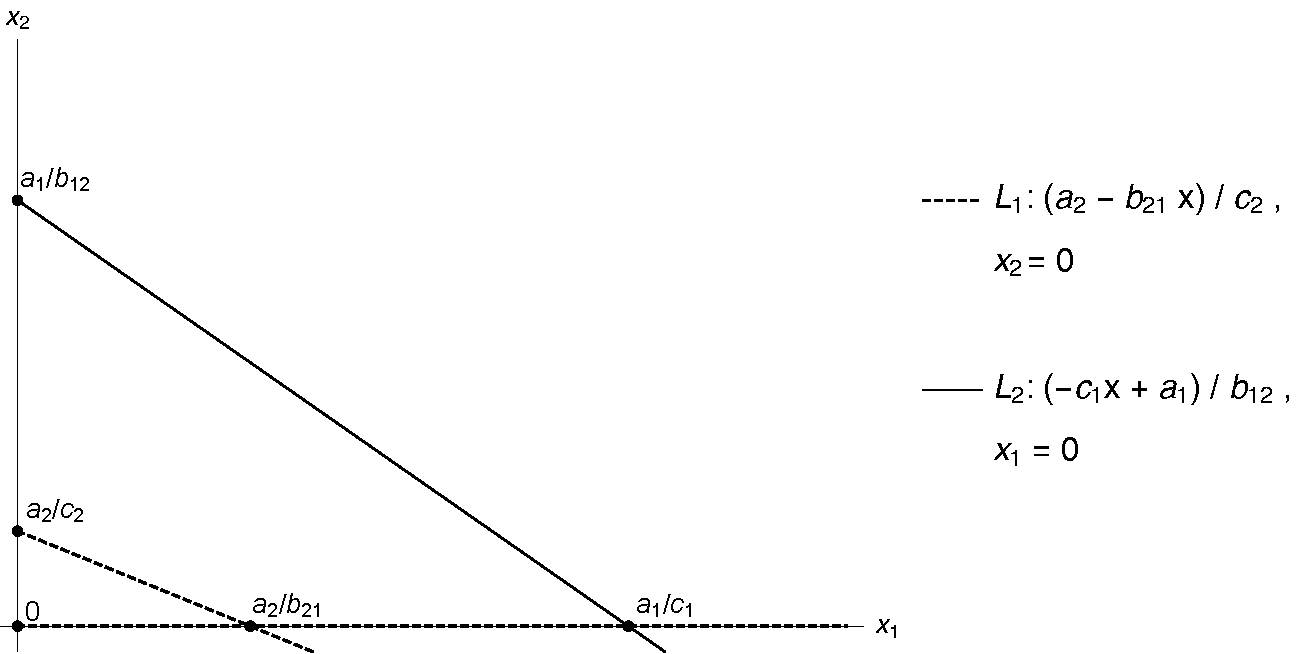
\includegraphics[width=0.95\textwidth]{sep_3.pdf}
        \caption{Первый дополниетльный случай расположения сепаратрис}
        \label{fig:sep_3}
    \end{figure}
    \begin{enumerate}
        \setlength\itemsep{0.5em}
        \item $ \lambda_1 = a_1 > 0,\ \lambda_2 = a_2 > 0 \Rightarrow $ точка $ (0, 0) $ --- неустойчивый узел.
    
        \item $ \lambda_1 = -a_1 < 0,\ \lambda_2 = \dfrac{a_2 c_1 - a_1 b_{21}}{c_1} < 0 \Rightarrow $ точка $ \left( \dfrac{a_1}{c_1}, 0 \right) $ --- устойчивый узел.
        
        \item  $ \lambda_1 = \dfrac{a_1 c_2 - b_{12} a_2}{c_2} > 0,\ \lambda_2 = -a_2 < 0 \Rightarrow $ точка $ \left( 0, \dfrac{a_2}{c_2} \right) $ --- седло.
        \\[0.05em]
    \end{enumerate}

    Проанализируем поля направлений:

    \begin{itemize}
        \setlength\itemsep{0.4em}
        \item В первой области $ \dot x_1 > 0 $ и $ \dot x_2 > 0 \, \Rightarrow $ траектории направлены вправо вверх.
        \item Во второй области $ \dot x_1 > 0 $ и $ \dot x_2 < 0 \, \Rightarrow $ траектории направлены право вниз.
        \item В третьей области $ \dot x_1 < 0 $ и $ \dot x_2 < 0 \, \Rightarrow $ траектории направлены влево вниз.
    \end{itemize}

    \begin{figure}[h]
        \centering
        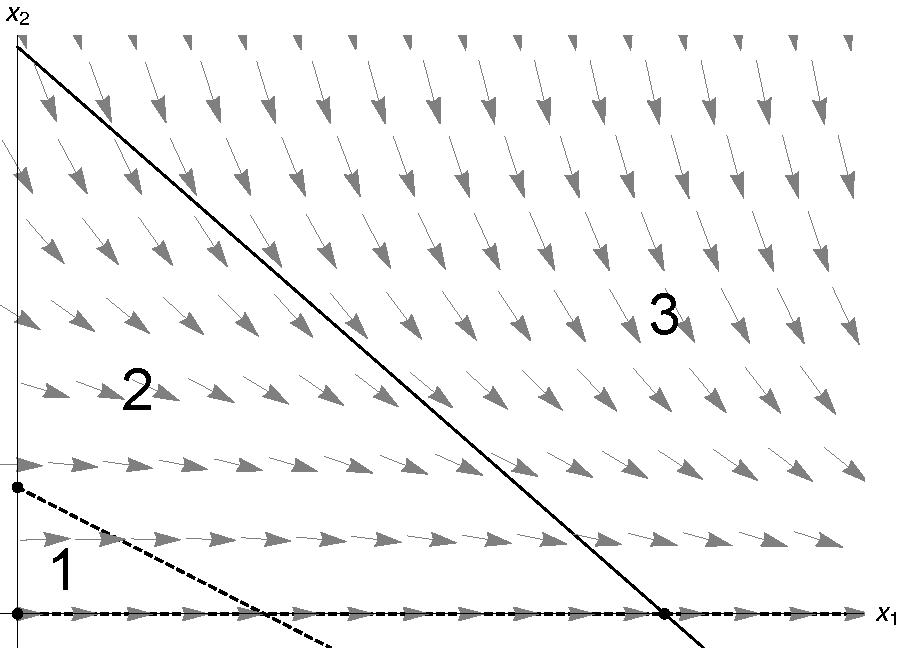
\includegraphics[width=0.7\textwidth]{dirFields_31.pdf}
        \caption{Поле направлений для $ \dot x_1 $}
        \label{fig:dirFields_31}
    \end{figure}

    \pagebreak

    \begin{figure}[h]
        \centering
        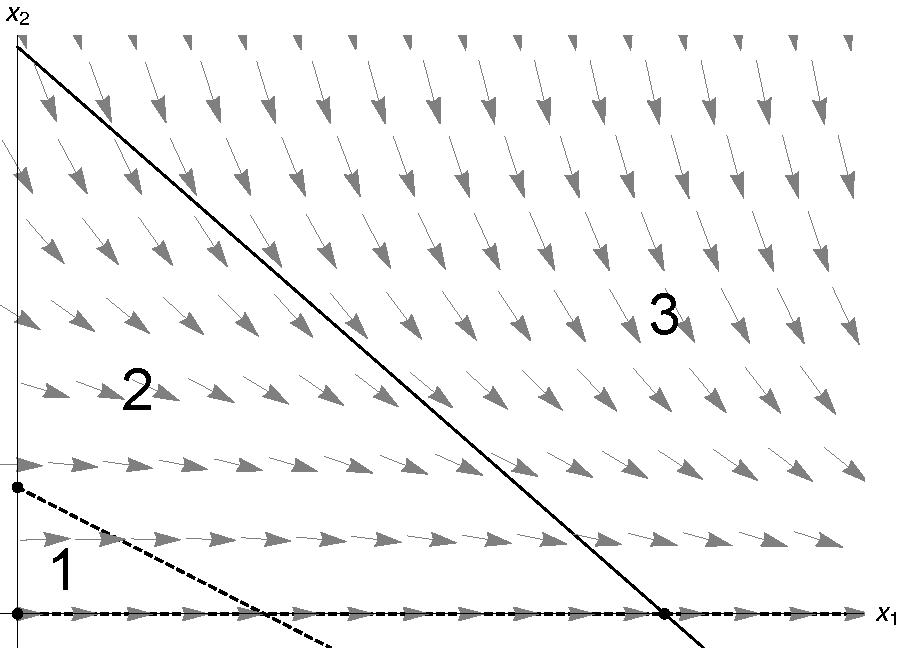
\includegraphics[width=0.64\textwidth]{dirFields_32.pdf}
        \caption{Поле направлений для $ \dot x_2 $}
        \label{fig:dirFields_32}
    \end{figure}
    
    \begin{figure}[h]
        \centering
        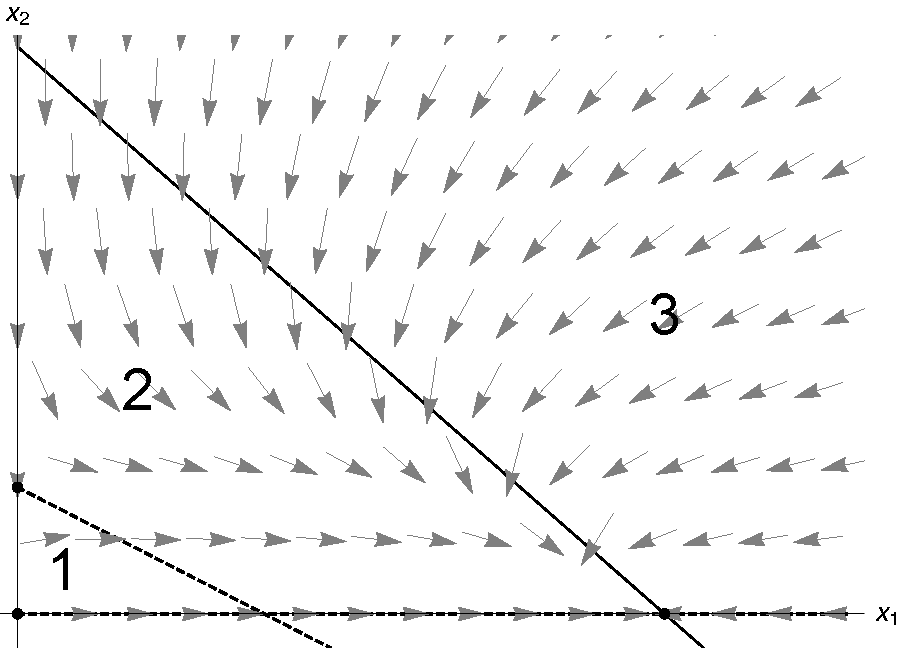
\includegraphics[width=0.64\textwidth]{areas_3.pdf}
        \caption{Общие направления траекторий}
        \label{fig:areas_3}
    \end{figure}

    \pagebreak

    Построим фазовый портрет для данного случая:
    \begin{figure}[h]
        \centering
        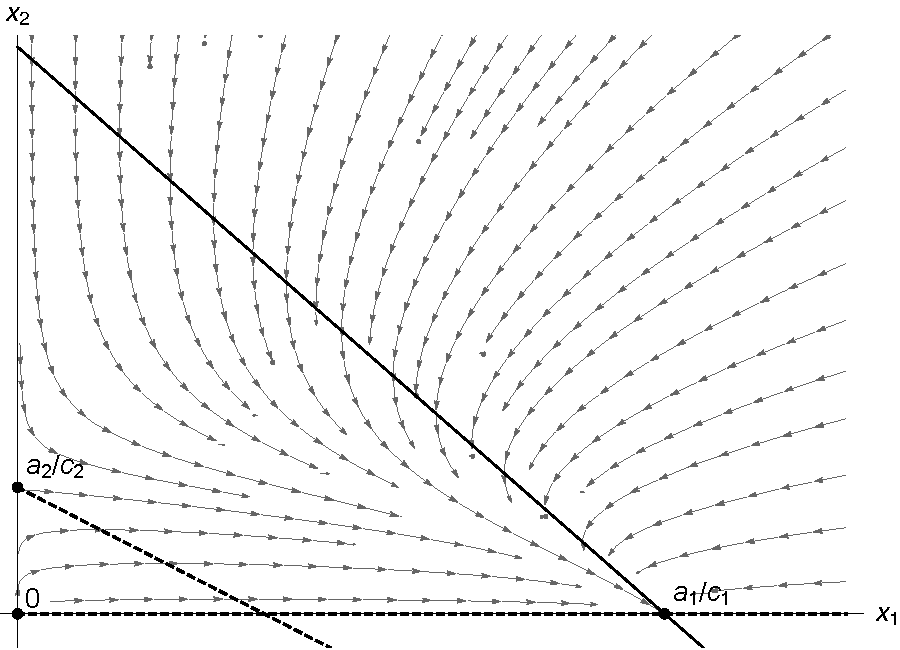
\includegraphics[width=0.64\textwidth]{phase_3.pdf}
        \caption{Выживает первый вид, второй --- вымирает}
        \label{fig:phase_3}
    \end{figure}
    
    В системе присутствует всего одно устойчивое состояние ($2^{\text{ая}}$ точка), поэтому все фазовые траектории стремятся к нему.

    \subsection{Второй случай}
    В случае выполнения условий \eqref{negpos} возникает противоположная ситуация:
    \begin{figure}[h]
        \centering
        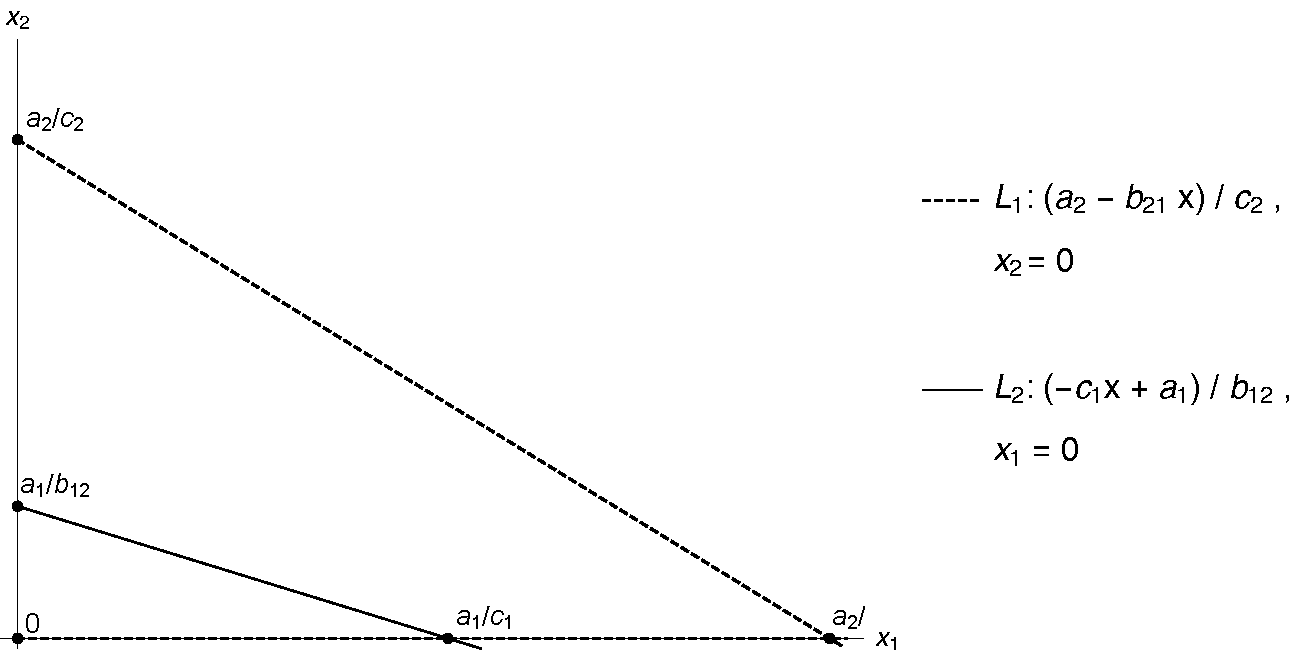
\includegraphics[width=0.78\textwidth]{sep_4.pdf}
        \caption{Второй дополниетльный случай расположения сепаратрис}
        \label{fig:sep_4}
    \end{figure}

    \begin{enumerate}
        \setlength\itemsep{0.5em}
        \item $ \lambda_1 = a_1 > 0,\ \lambda_2 = a_2 > 0 \Rightarrow $ точка $ (0, 0) $ --- неустойчивый узел.
    
        \item $ \lambda_1 = -a_1 < 0,\ \lambda_2 = \dfrac{a_2 c_1 - a_1 b_{21}}{c_1} > 0 \Rightarrow $ точка $ \left( \dfrac{a_1}{c_1}, 0 \right) $ --- седло.
        
        \item  $ \lambda_1 = \dfrac{a_1 c_2 - b_{12} a_2}{c_2} < 0,\ \lambda_2 = -a_2 < 0 \Rightarrow $ точка $ \left( 0, \dfrac{a_2}{c_2} \right) $ --- устойчивый узел.
    \end{enumerate}

    Поля направлений: 

    \begin{itemize}
        \setlength\itemsep{0.4em}
        \item В первой области $ \dot x_1 > 0 $ и $ \dot x_2 > 0 \, \Rightarrow $ траектории направлены вправо вверх.
        \item Во второй области $ \dot x_1 < 0 $ и $ \dot x_2 > 0 \, \Rightarrow $ траектории направлены влево вверх.
        \item В третьей области $ \dot x_1 < 0 $ и $ \dot x_2 < 0 \, \Rightarrow $ траектории направлены влево вниз.
    \end{itemize}

    \begin{figure}[h]
        \centering
        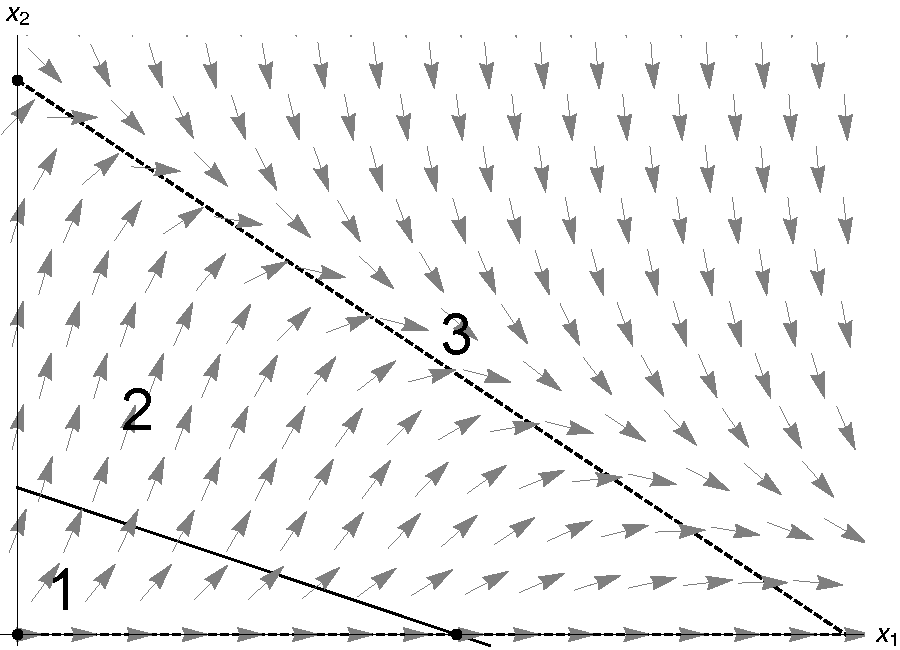
\includegraphics[width=0.7\textwidth]{dirFields_41.pdf}
        \caption{Поле направлений для $ \dot x_1 $}
        \label{fig:dirFields_41}
    \end{figure}

    \pagebreak

    \begin{figure}[h]
        \centering
        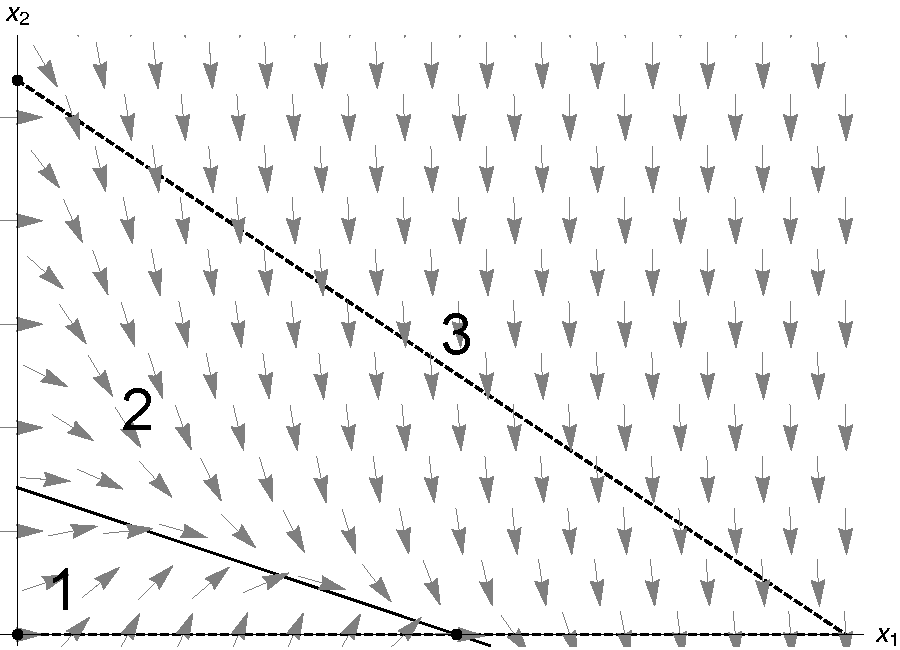
\includegraphics[width=0.64\textwidth]{dirFields_42.pdf}
        \caption{Поле направлений для $ \dot x_2 $}
        \label{fig:dirFields_42}
    \end{figure}
    
    \begin{figure}[h]
        \centering
        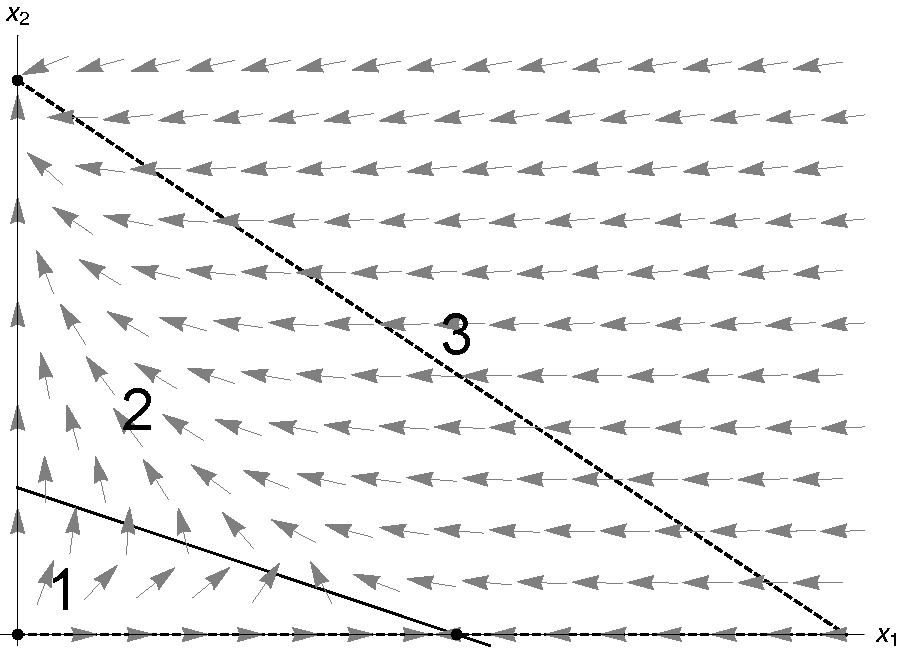
\includegraphics[width=0.64\textwidth]{areas_4.pdf}
        \caption{Общие направления траекторий}
        \label{fig:areas_4}
    \end{figure}

    \pagebreak

    Фазовый портрет с учетом всего выше сказанного:
    \begin{figure}[h]
        \centering
        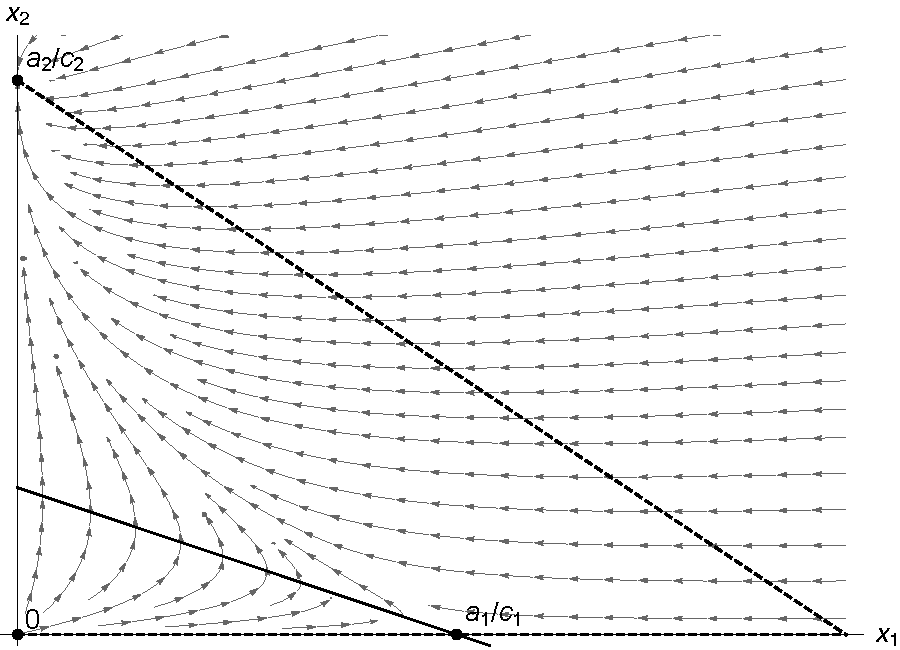
\includegraphics[width=0.75\textwidth]{phase_4.pdf}
        \caption{Выживает второй вид, первый --- вымирает}
        \label{fig:phase_4}
    \end{figure}
    
    Как и в предыдущем случае, в системе присутствует одно устойчивое состояние, однако на этот раз оно соответствует $1^{\text{ой}}$ точке, и все траектории устремляются к ней.

    \section-{Заключение}
    Имея экспериментально выведенные коэфициенты размножения, а также коэфициенты межвидовой и внутривидовой конкуренции, мы можем построить модель взаимодействия между особями двух видов и понять, способны ли они сосуществовать или же один из них вымрет. Анализ особых точек (иными словами --- стационарных состояний) дает нам возможность построить график траекторий, чтобы определить, к какому из четырех стационарных состояний стремится система.

    \newpage

    \begin{thebibliography}{9}
        % \bibitem{Loyts} Лойцянский Л.\,Г. Механика жидкости и газа. М.: Дрофа, 2003. 846 с.

        \bibitem{Model} Ризниченко Г.\,Ю. Лекции по математическим моделям в биологии. --- 2-е изд. испр. и доп. --- М. --- Ижевск: Институт компьютерных исследований, НИЦ <<Регулярная и хаотическая динамика>>. 2010. 560 с.

        \bibitem{agafonov} Агафонов С.А., Герман А.Д., Муратова Т.В. Дифференциальные уравнения. М.: Изд-во МГТУ им. Н.Э. Баумана, 1997. 336 с.

        \bibitem{petrovsky} Петровский И.Г. Лекции по теории обыкновенных дифференциальных уравнений. М.: Наука. 1970. 280 с.

        \bibitem{pentryagin} Понтрягин Л.С. Обыкновенные дифференциальные уравнения. М.: Наука. 1970. 332 с.

        \bibitem{samarsky} Самарский А.А., Гулин А.В. Численные методы. М.: Наука: Физматлит, 1989. 416 с.

    \end{thebibliography}

    \end{document}